\chapter{Sediment Transport in the German Coastal Baltic Sea}
\label{kap-measure}

This study addresses the question whether the deep basins in the Baltic Sea are 
purely depositional or if sediment once settled there can be transported back 
to shallower areas. Field data, including long-term moorings and 
microstructure measurements, from three cruises in three different years 
and seasons has therefore been analyzed to investigate mean current, turbulence 
and suspended sediment concentration. Measurements have been carried out on the 
transition zone from the German shore to the Arkona basin. It is found that 
net onshore transport of suspended matter originating from the Arkona basin 
takes place. Stratification asymmetries in the flow phases of an oscillatory 
up- and down-slope flow have been identified as a possible mechanism for this 
net sediment transport.

\section{Introduction}

The investigation of sediment transport patterns and the physical processes 
involved is inevitable for the understanding and mapping of all near bottom 
biogeochemical processes. Nutrients as well as pollutants are distributed or 
accumulated together with the sediment and affect benthic communities and the 
exchange of dissolved substances from pore water with the overlying water. 
Especially in coastal areas, a broad variety of hydrodynamical processes affect 
resuspension, transport and accumulation of sediments. In very shallow areas, 
wind waves govern the sediment dynamics, whilst mean flow, near bottom 
turbulence and interior stratification becomes more and more important on the 
transition to the deeper areas further away from the coast.

In the presence of only negligible tidal motions, coastal areas of the Baltic 
Sea are a good opportunity to study the interplay of waves and currents and its 
effects on sediment transport patterns. Numerous studies have already been 
carried out to investigate suspended matter transport in the German Baltic Sea. 
In the \textit{Ba}ltic Sea \textit{Sy}stem \textit{S}tudy (BASYS) project, the 
pathways of fine-grained sediment from the near-shore regions to the deep 
basins were investigated with the help of numerical models and ship-based 
measurements \citep[][]{basys1, basys2, leipe2000}. The research project 
\textit{Dynamic} of \textit{N}atural and \textit{A}nthropogenic 
\textit{S}edimentation (DYNAS) investigated the spatially resolved 
resuspension and transport patterns in the whole near-coastal area of the 
south-western Baltic Sea, using a numerical model 
\citep[][]{dynas1, dynas2}. These studies, amongst many others, focus mainly on 
the large scale sediment transport and aim to identify erosional and 
depositional areas of the sea floor. 

The small-scale turbulent motions, which are an important factor for sediment 
transport processes, have not been included in the projects mentioned above. 
They affect the bottom shear stress that causes resuspension and determine how 
suspended matter is mixed up in the water column. In the interdisciplinary 
project The \textit{Se}rvice of sediments in German \textit{Co}stal 
\textit{S}eas (SECOS), during which the present study is carried out, these 
small-scale processes are examined with an extensive field work campaign. This 
included ship-based micro-structure measurements and long-term mooring 
deployments. With the combined measurement of suspended matter concentration 
using optical backscatter sensors and mean flow structures as well as turbulent 
motions we aim on determining the relative effect turbulence has in 
resuspension and distribution of sediment. 

One of the most interesting regions where measurements were carried out was the 
transition zone from near-coast to a deeper basin north of the island 
R\"{u}gen. This can be regarded as a prototype study side, as it covers shallow 
as well as deeper areas, which are affected by waves to different extends, and 
it includes the basin structure of the Baltic Sea. To our knowledge, 
no turbulence measurements with focus on sediment dynamics were carried out in 
this region so far.
 
In addition, this area provides the prerequisites for the occurrence of 
slope-induced tidal straining \citep[][]{UmlaufBurchard2011a, 
schulzumlauf2016}, as visible in Fig.\ \ref{abslope}. Both slope angle and 
interior vertical stratification are sufficient to trigger residual sediment 
transport under an oscillatory current. Although tides are negligible in the 
Baltic Sea, we discovered a distinct signal of inertial oscillations with a 
period of approximately 17~h over the whole time of a five day continuous 
current measurement. This setting surely exceeds the capability of the 
one-dimensional numerical model used in \cite{schulzumlauf2016}, as the slope 
angle changes and the vertical stratification is greatly enhanced in the 
region of the halocline, making the problem at least two-dimensional. 
Nevertheless, sediment transport from the basin up the slope could be induced 
by slope-induced tidal straining under the conditions given in this region.

 \begin{figure}[ht]
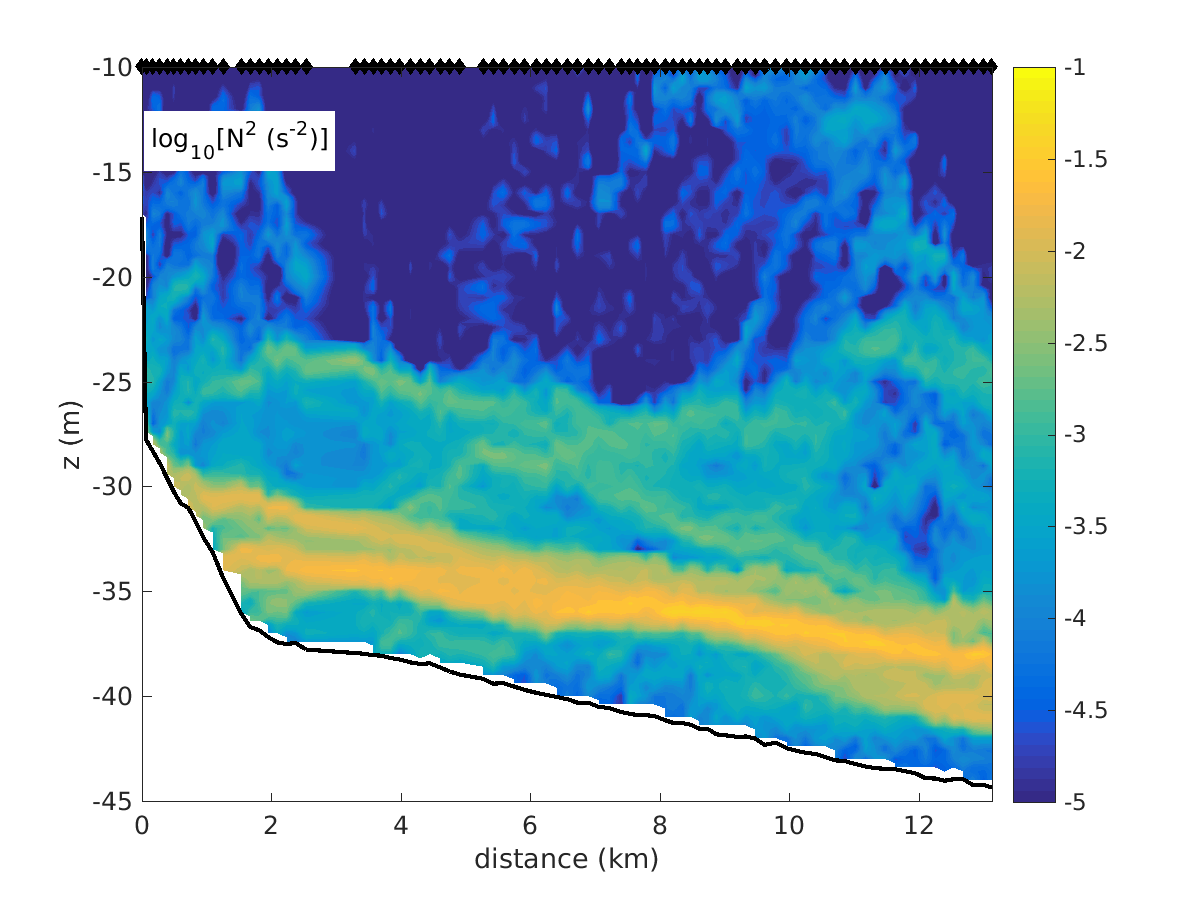
\includegraphics[width=40pc]{bilder/abslope.png}
 \caption{(b) Topographic and hydrologic structure in the study area 
obtained from microstructure transect T1 (see Tab.\ \ref{mss} and Fig.\ 
\ref{studyarea}) in 2016. The steep slope on the left hand side has an 
inclination of approximately $5 \times 10^{-3}$, the mild slope further to the 
right of around $7 \times 10^{-4}$. Color indicates the buoyancy frequency 
$N^2$. In (a), ca. five days of the cross-slope (i.e. southward) near-bottom 
current are displayed, obtained with a 1200~kHz ADCP in April 2014 (see Tab.\ 
\ref{deployments}, first column.)}
 \label{abslope}
 \end{figure}
 
 The deep basins in the Baltic Sea, like the Arkona basin, are depositional 
areas. Net sedimentation can be measured, and sediment is transported from the 
coast to the basins \citep[][]{basys1, basys2}. The main question we adress in 
this study is whether this transport is directed purely one way, or if processes 
exist which can transport parts of the sediment from the deep basins back to 
shallower areas.

\section{Study Area}

The general properties of the Baltic Sea have already been discussed in the 
last chapter. Here, we give a brief introduction to the general hydrodynamic 
processes which govern the current system near the measurement site on the one 
hand, and the sediment distribution on the other.

\subsection{Hydrology}

In \fig{studyarea}, the bathymetry of the study area and its position in the 
Western Baltic Sea is displayed. The flow patterns in this area have already 
been investigated with extensive field measurement e.g. in \cite{lass1993}. In 
a study on the Pomeranian Bight (i.e. the shallow area connecting the Arkona 
Basin in the west and the Bornholm Basin in the east and where the mouth of the 
Oder river is located), \cite{lass2001} also investigated the study site 
described here both observationally and with a high-resolution circulation 
model. In addition, the same authors carried out measurements in two consecutive 
winters in the Arkona Basin and analyzed the flow dynamics there 
\citep[][]{lass2003}. These three studies give a good insight 
of the flow patterns in the area where our investigations were performed.
 
 \begin{figure}[ht]
 \centering
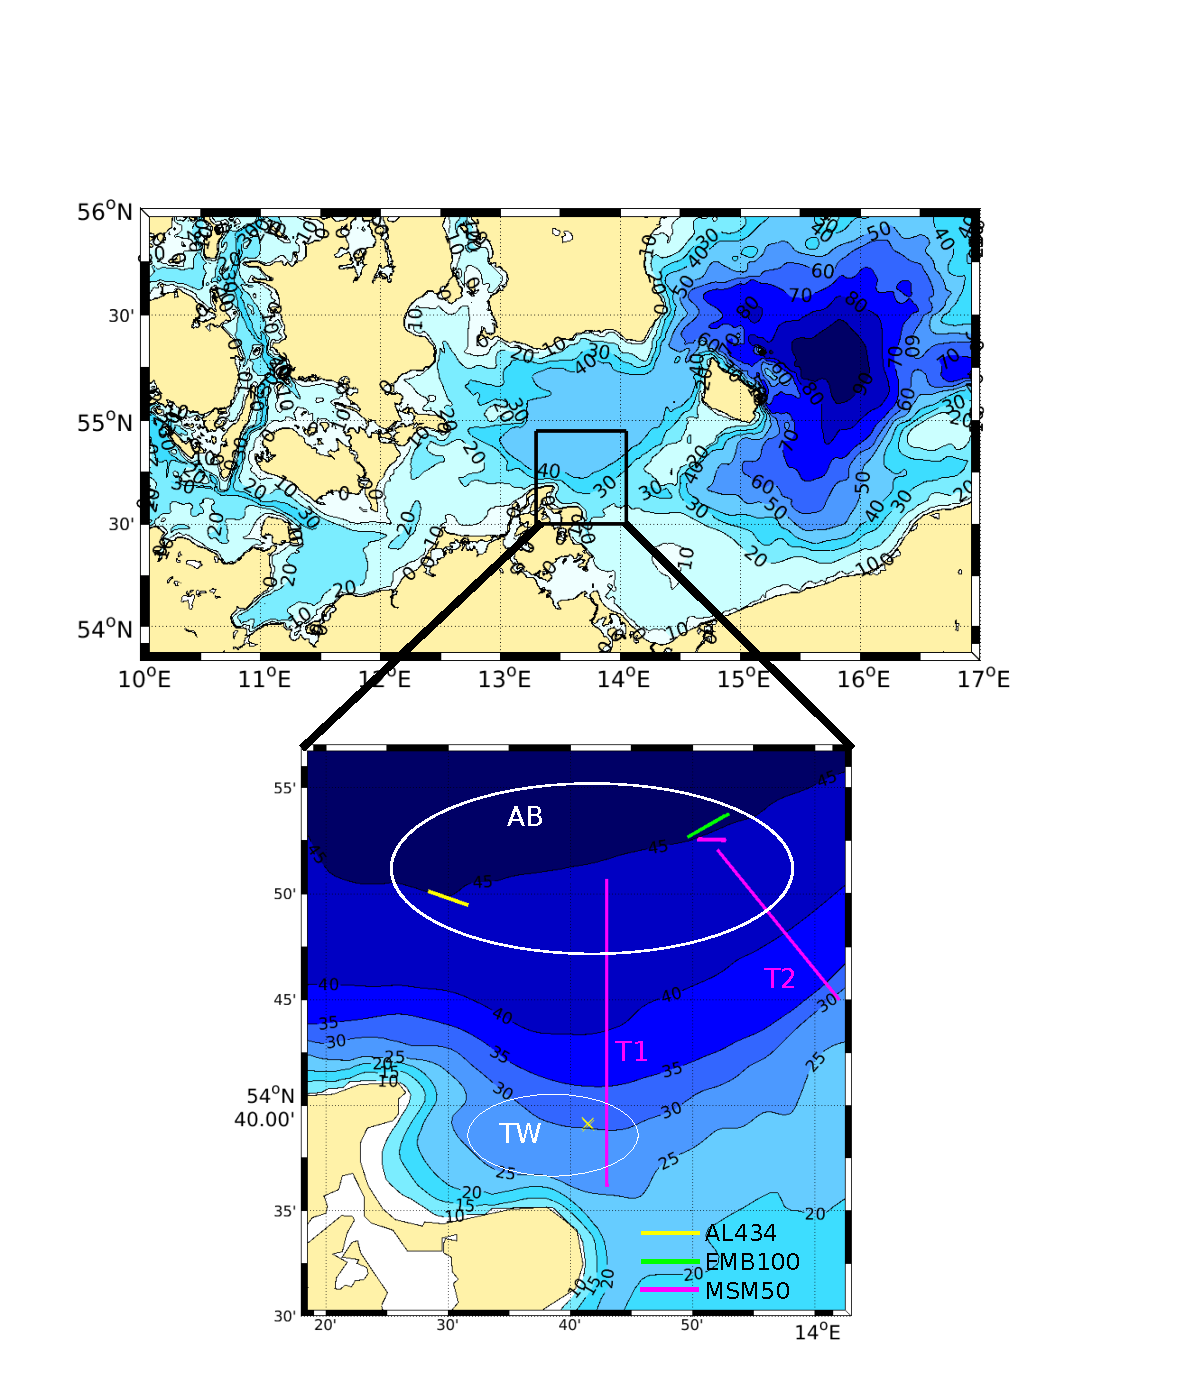
\includegraphics[width=18cm]{bilder/studyarea.pdf}
 \caption{Bathymetric map of the Western Baltic Sea and an enlargement of the 
study area. Deployments during cruise AL434 are indicated in yellow, from 
EMB100 in green and from cruise MSM50 in magenta.}
 \label{studyarea}
 \end{figure}

Two main drivers are determining the currents. From the exchange with the North 
Sea, dense bottom currents of saline water flows into the Arkona Basin. 
Coriolis effects form a topographically trapped dense rim current which rotates 
cyclonically around the basin, following the slope. As inflow events are 
driven by larger scale wind forcing, this process is not steady, and the 
dense bottom current can disappear completely. Parts of the saline bottom water 
are transferred from the cyclonic bottom current to the saline bottom water 
pool, which fills approximately the lowermost 15~m of the basin. The barotropic 
cyclonic motion performs basin wide zonal oscillations on timescales of one 
week \citep[][]{lass2003}.

Near-shore currents reveal an elliptical motions, with the main axis 
being aligned along the isobaths \citep[][]{lass2003}. North of the island 
R\"{u}gen, the currents are slightly more pronounced towards the east. The 
cross-shore component is generally weaker, but still in the order of 
0.1~m~s$^{-1}$ \citep[][]{lass1993}. 

The other main factor determining the flow conditions is local wind forcing, 
that causes upwelling and downwelling near the shore. Wind from the east drives 
a long-shore current to the west. In cross-shore direction, Ekman 
transport causes surface flow to be directed seaward. This induces a 
near-bottom return current towards the land \citep[][]{lass1993}. The salt 
water pool in the Arkona basin is consequently tilted upwards towards the 
southern rim of the basin \citep[][]{lass2003}. During wind from the west, the 
situation is reversed. 

 \FloatBarrier
\subsection{Sedimentology}

  Sediment distribution in this area is heterogeneous in the shallow regions 
with predominately medium to fine sand. At water depths below 25 - 30~m in the 
Arkona Basin, sediment is finer and consists homogeneously of silt 
(\fig{tauberkarte}). In the vicinity of TW, a special type of fine grained and 
organic poor sediment is found. Previous studies \citep[][]{leipe2000, 
basys1} found the Arkona Basin to be a deposition center for material 
orginiating from the shallower areas, with accumulation rates of around 2.2 
mm/yr. Sediment characteristics in the Arkona Basin resemble to those of a 
fluffy layer, i.e. it is easily resuspended and, due to its low settling 
velocity, remains suspended for a relatively long period of time. A consecutive 
study \citep[][]{basys2} found the 20~m isobath to be the border between 
erosional and depositional sites in this area, yielding that the Tromper Wiek 
region is depositional as well. This study also pointed out that muddy 
sediments accumulated below the halocline in this region.
 \begin{figure}[ht]
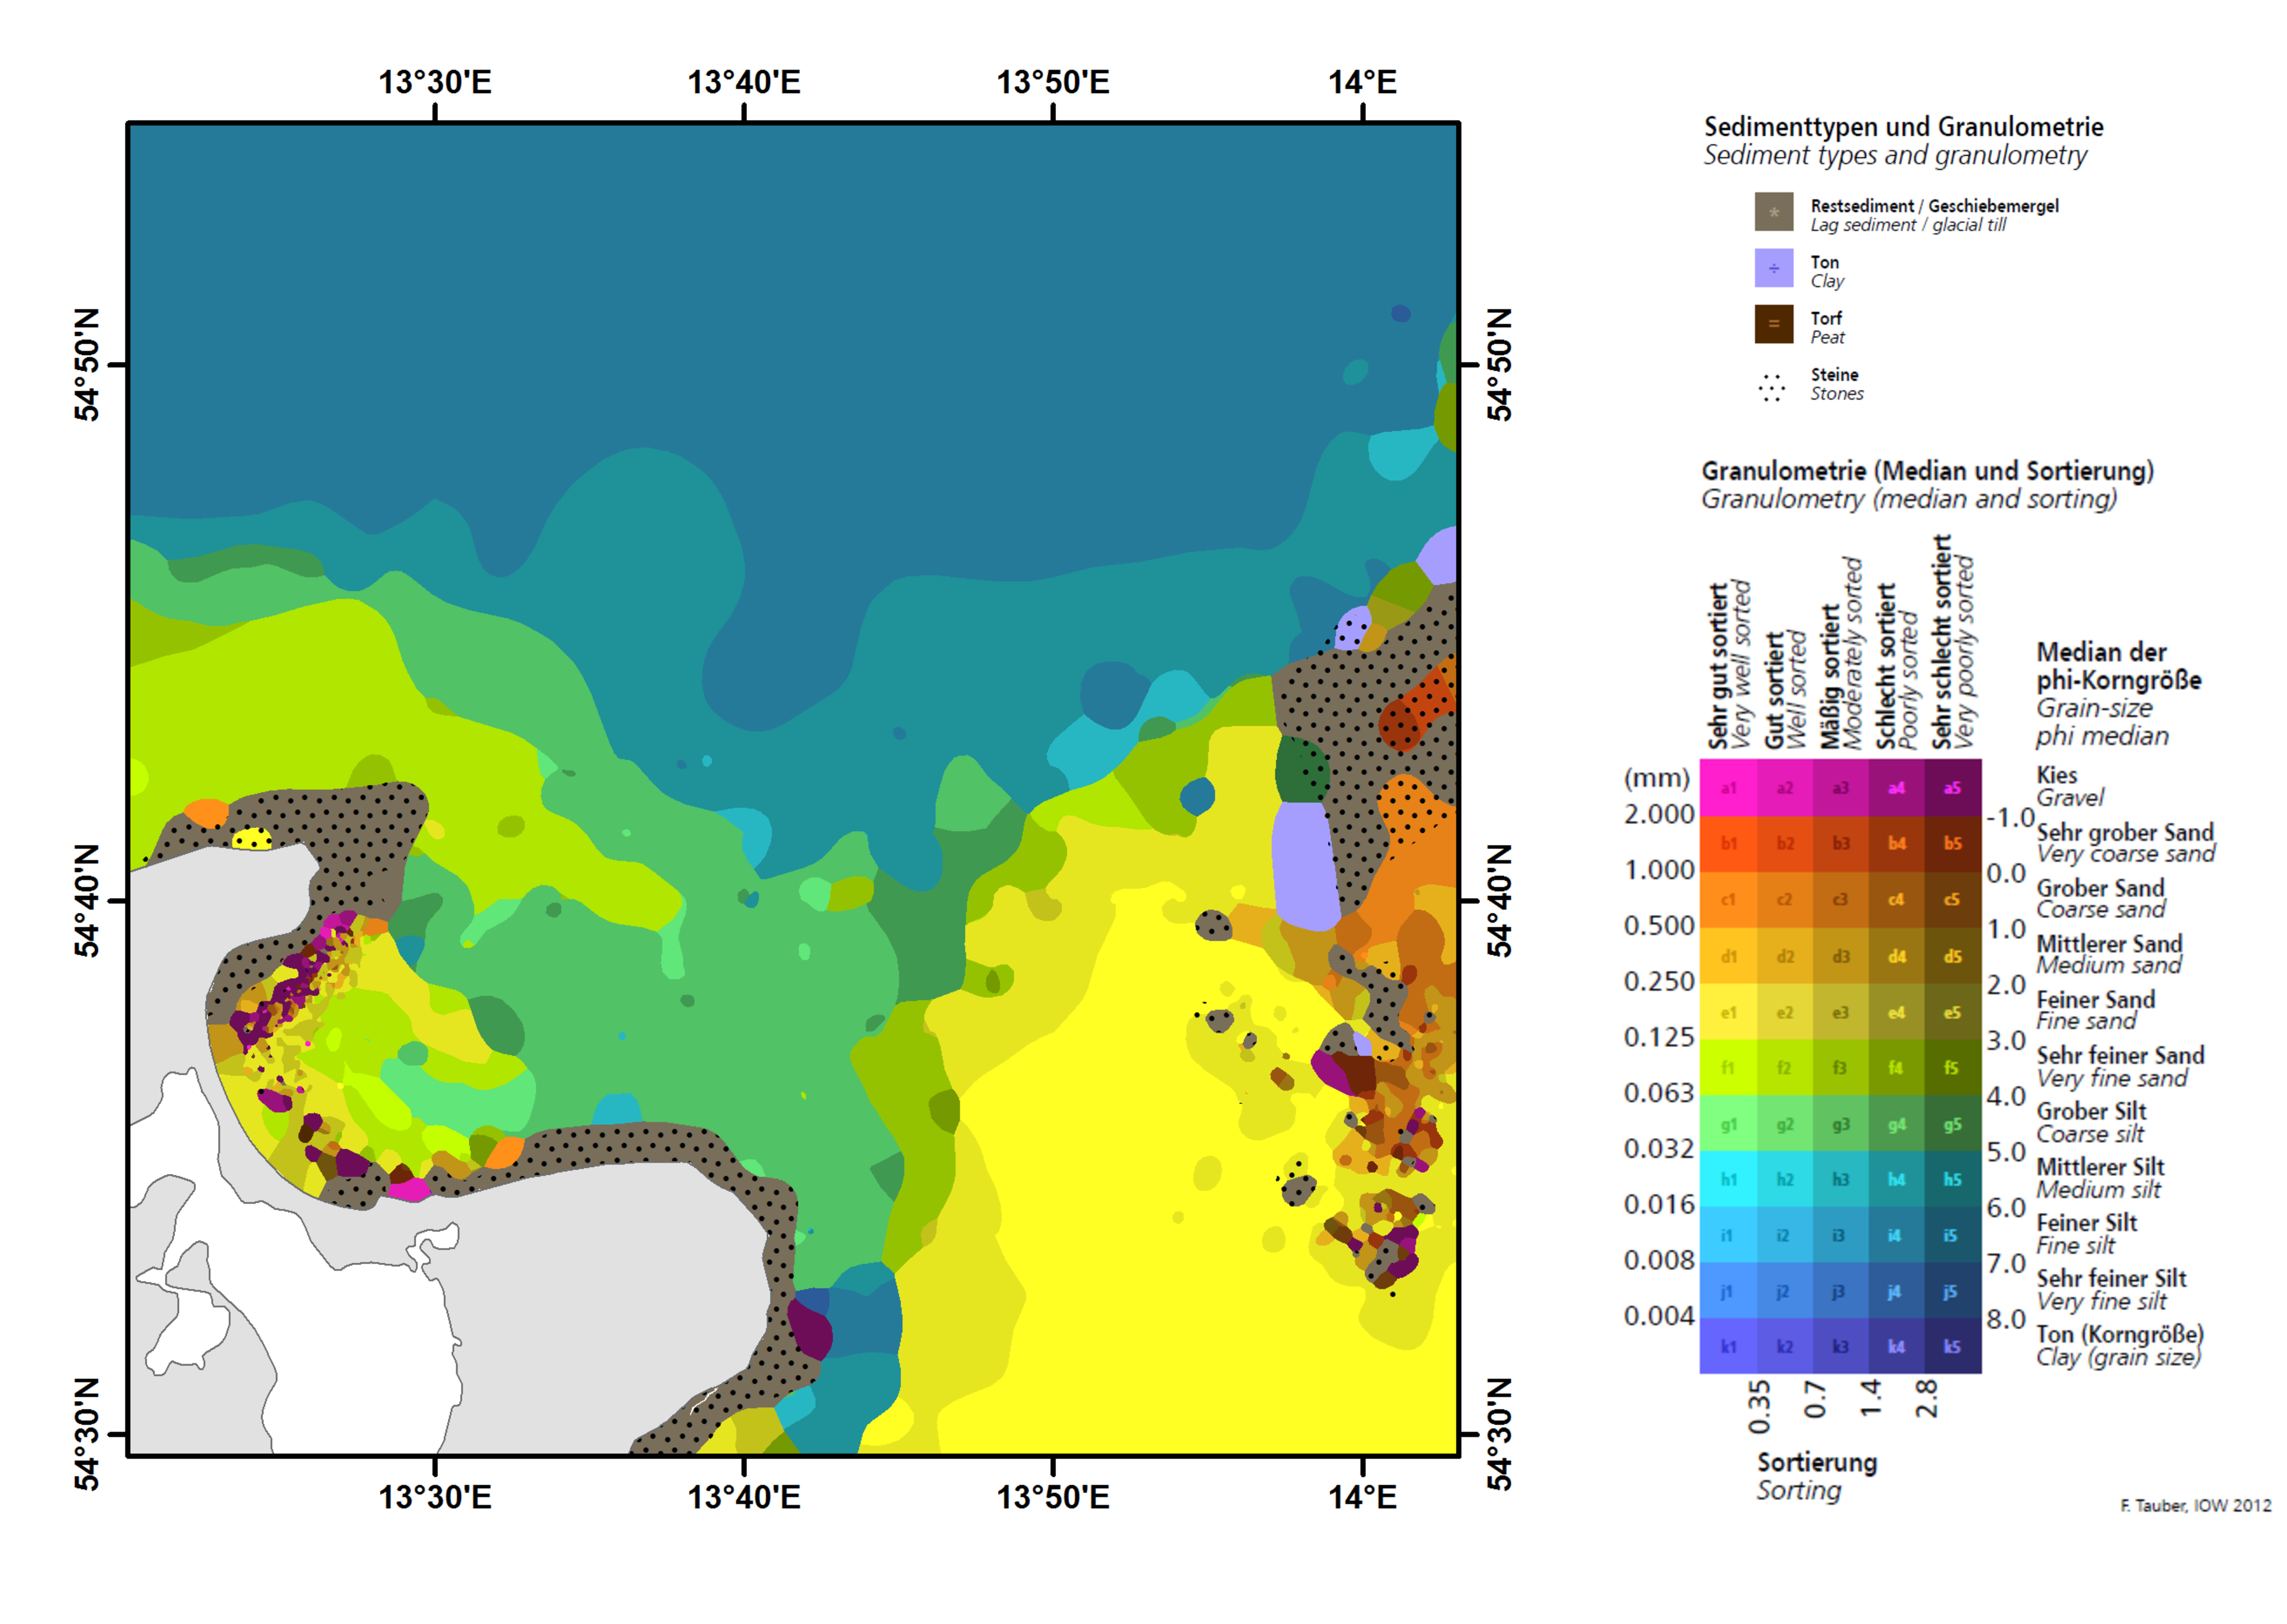
\includegraphics[width=30pc]{bilder/TW.pdf}
 \caption{Sediment distribution in the study area. Data were taken from 
\cite{tauber2012}.}
 \label{tauberkarte}
 \end{figure}

\section{Instrumentation}

We obtained hydrographic and turbulence data at 
several locations throughout the German coastal area during three cruises with 
R/V \textit{Alkor} in spring 2014 (AL434, 28.03.-08.04.2014), R/V 
\textit{Elisabeth Mann Borgese} in spring 2015 (EMB100, 09.04.-16.04.2015) and 
R/V \textit{Maria S. Merian} in winter 2016 (MSM50, 05.01.-29.01.2016). Here, 
we exclusively discuss data obtained in the transition zone from the coast off 
the island R\"{u}gen (called Tromper Wiek (TW), around 30~m water depth) to 
the approximately 45~m deep Arkona Basin (AB). The exact positions of deployed 
moorings and ship-based microstructure profiler transects are indicated in 
\fig{studyarea}.

Three different types of moorings were deployed: A CTD-Chain consisted of eight 
CTD-loggers (MicroCat from Seabird, USA), tied to a mooring line at intervals 
of 1 m, starting at 1 m above the seabed, additionally two optical 
backscatter sensors (NTU from Wetlabs, USA) at 3.5 and 5.5 m above the seabed. 
For the EMB100 cruise, the CTD-Chain was extended to 10 CTD-loggers (5 MicroCat 
and 5 TR-1060 type from RBR, Canada) and the turbidity sensors were omitted. 
Lander 1 was a bottom-mounted instrument frame with an upward looking 1200 kHz 
ADCP (Teledyne RDI, USA), a 6 MHz single-point Doppler current meter (Vector 
from Nortek AS, Norway), another CTD-logger and a turbidity sensor. Lander 2 
was a similar bottom frame equipped with an upward looking 600 MHz ADCP 
(Teledyne RDI, USA) and an upward looking 1 MHz (2 MHz during cruise AL434) 
pulse-coherent ADCP (Aquadopp HR from Nortek AS, Norway). For the cruises 
EMB100 and MSM50, Lander 2 was complemented with an additional CTD-logger and a 
turbidity sensor. Deployment times of the moorings are listed in 
\tab{deployments}.

 \begin{table}
\caption{Deployment times of moorings (UTC). In the first 
line, TW and AB indicate deployment sites near the coast and in the Arkona 
Basin, respectively.}\label{deployments}
\begin{center}
\begin{tabular}{cccc}
 & AL434 (TW) & EMB100 (AB) & MSM50 (TW) \\
 \hline
 start & 03.04.2014, 07:00 & 14.04.2015, 12:00 & 26.01.2016, 22:00 \\ 
 end & 08.04.2014, 06:00 & 17.04.2015 04:00 & 28.01.2016, 07:00 \\
\hline
 & CTD-Chain & CTD-Chain & \\
 & Lander 1 & Lander 1 & Lander 1\\
 & Lander 2 & Lander 2 & Lander 2\\
\end{tabular}
\end{center}
\end{table}

Ship-based microstructure measurements were performed with a MSS90-L 
microstructure profiler (ISW, Germany). The instrument contained a set of 
precision CTD sensors, a fast FP07 thermistor, a turbidity sensor, and two 
airfoil shear-probes. During the transects (each of 1 to 5 hours duration) the 
ship moved at 1-2 kn and profiles were obtained continously. Number and time of 
the transects for each cruise are summarized in \tab{mss}.

 \begin{table}
\caption{Start and end times (UTC) and number (in brackets) of microstructure 
transects.}\label{mss}
\begin{center}
\begin{tabular}{cccc}
 & AL434 (2014) & EMB100 (2015) & MSM50 (2016)\\
 \hline
Tromper & 04.04., 16:15 - & & 27.01., 00:00 - \\ 
Wiek & 04.04., 22:30 (4) & & 28.01., 06:00 (9)\\
 & 06.04., 17:30 & & \\
 &  07.04., 22:15 (8) & & \\
\hline
Arkona & 05.04., 16:15 - & 14.04., 16:45 - & 23.01., 13:30 - \\
Basin & 06.04., 01:15 (5) & 15.04., 05:30 (5) & 24.01., 16:45 (7)\\
\hline
transect &  & & 24.01., 19:30 - 23:45 (T1)\\
coast to basin & & & 28.01., 09:45 - 17:00 (T2)\\
\end{tabular}
\end{center}
\end{table}

\section{Observations}

\subsection{Tromper Wiek}

During the 5 day instrument deployment in 2014 (\tab{deployments}), we captured 
a storm event with 7 Bft wind and up to 4 m wave height with a consecutive calm 
period (\fig{tromperwiek}, a). In \fig{tromperwiek}, b the variance of the 
horizontal velocity componentsfiltered for wave periods between 2 and 20 
seconds, which is proportional to the kinetic energy contained in the 
waves, is displayed. Although wave energy was maximal in the afternoon of April 
4, the peak in turbidity was not reached until late morning of April, 5. This 
yields that local resuspension during storm did not occur, but a turbid 
watermass was advected to the measurement site. Near bottom current 
(\fig{tromperwiek},c) was directed to the south during the relevant period, 
i.e. water from deeper parts was advected up the slope.

 \begin{figure}[ht]
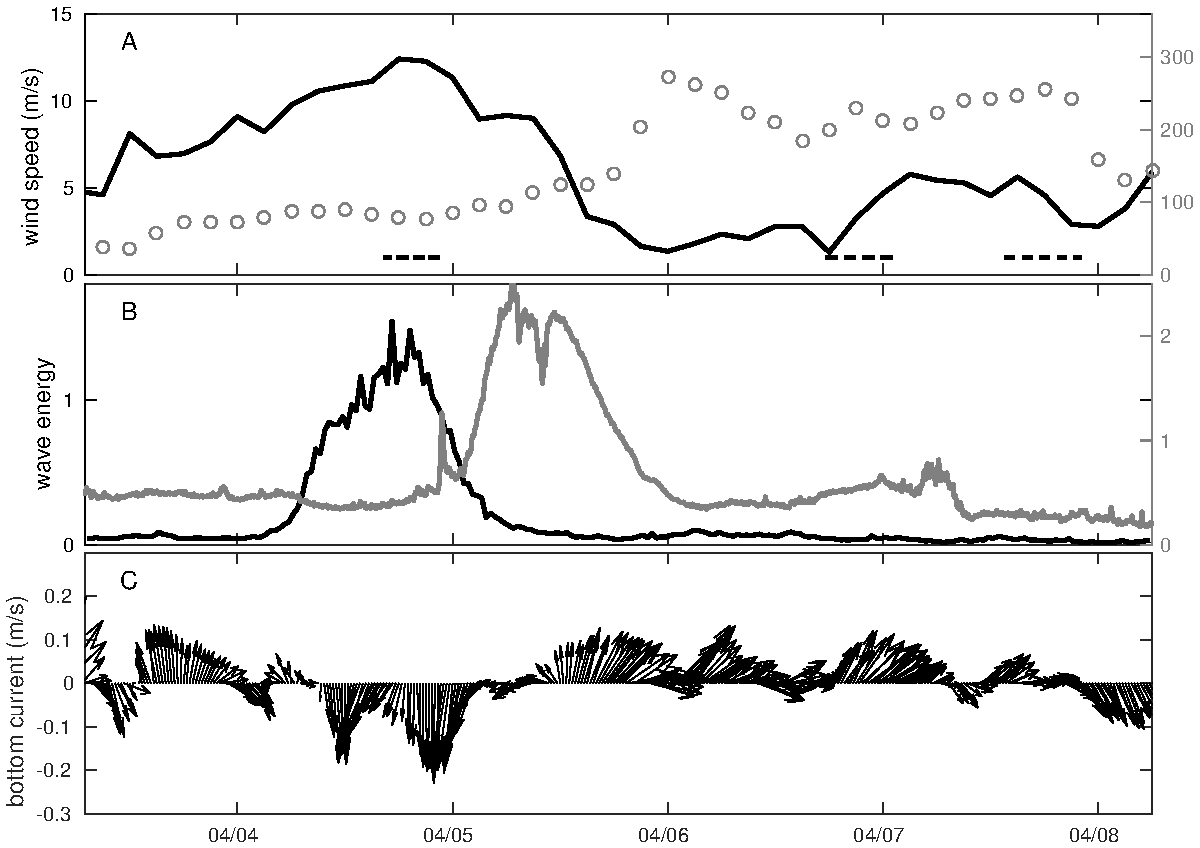
\includegraphics[width=15cm]{bilder/al434tw.pdf}
 \caption{(A) Wind speed and direction from the hindcast of the German Weather 
Service, (B) wave energy and turbidity and (C) direction of 
near bottom current, all obtained with Lander 1 during the deployment at TW on 
cruise AL434 (April 2014).}
 \label{tromperwiek}
 \end{figure}
 
 This advection of saline water near the bottom is triggered by the local wind 
forcing. Strong easterly wind causes Ekman transport to the north (i.e. 
offshore) in the surface layer \citep[][]{lass2001}, which is visible in the 
velocity data from the 600~kHz ADCP mounted on Lander~2, displayed in 
\fig{adcp600}. The distorted values in the uppermost part of the water column 
during April 4 coincide with the periods of time during which surface waves 
could be recorded with the ADV. They originate from breaking waves which 
disrupt the acoustic velocity measurements. The near-bottom return current below 
17~m depth is rather oscillatory than steady, but exhibits a trend to southerly 
(i.e. onshore) directions during the storm. Maximal onshore bottom flow is 
reached by the beginning of April 5. After the wind decayed and changed 
direction to westerly wind at the end of April 5, the surface current 
firstly decayed and was then reversed to flow approximately southwards. The 
near-bottom current of the flow remained unsteady, but was generally directed 
eastwards. This is more clearly visible from \fig{tromperwiek},c.

 \begin{figure}[ht]
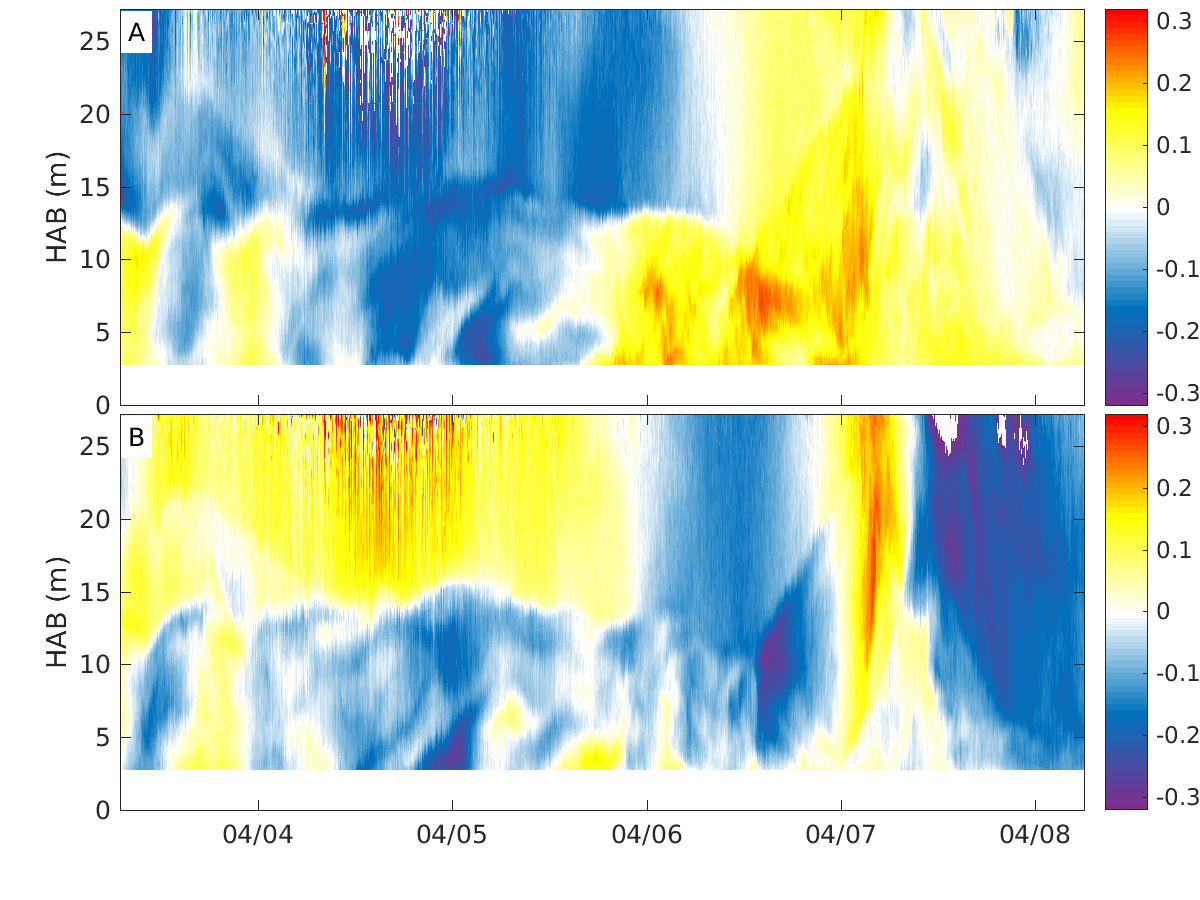
\includegraphics[width=40pc]{bilder/adcp600.png}
 \caption{Time series of velocity profiles obtained with the 600~kHz ADCP on 
Lander 2 during the deployment at TW on cruise AL434 (April 2014).}
 \label{adcp600}
 \end{figure}

 In the CTD Chain data in \fig{ctdchain}, where salinity in the lowermost 8~m 
of the water column is displayed, we see an increase of the 
near-bottom salinity, accompanied by increasing turbidity, starting in the 
afternoon of April 4. The increase in turbidity is clearly linked to the 
increase of salinity, supporting that turbid water is advected to TW from deeper 
regions. Furthermore, salinity data in the record reaches a level that 
resembles more to the saline bottom water in the Arkona basin below the 
halocline than to the brackish surface water. This indicates that upwelling 
tilted the halocline towards the south and saline bottom water reached far 
upslope to the shore.

 \begin{figure}[ht]
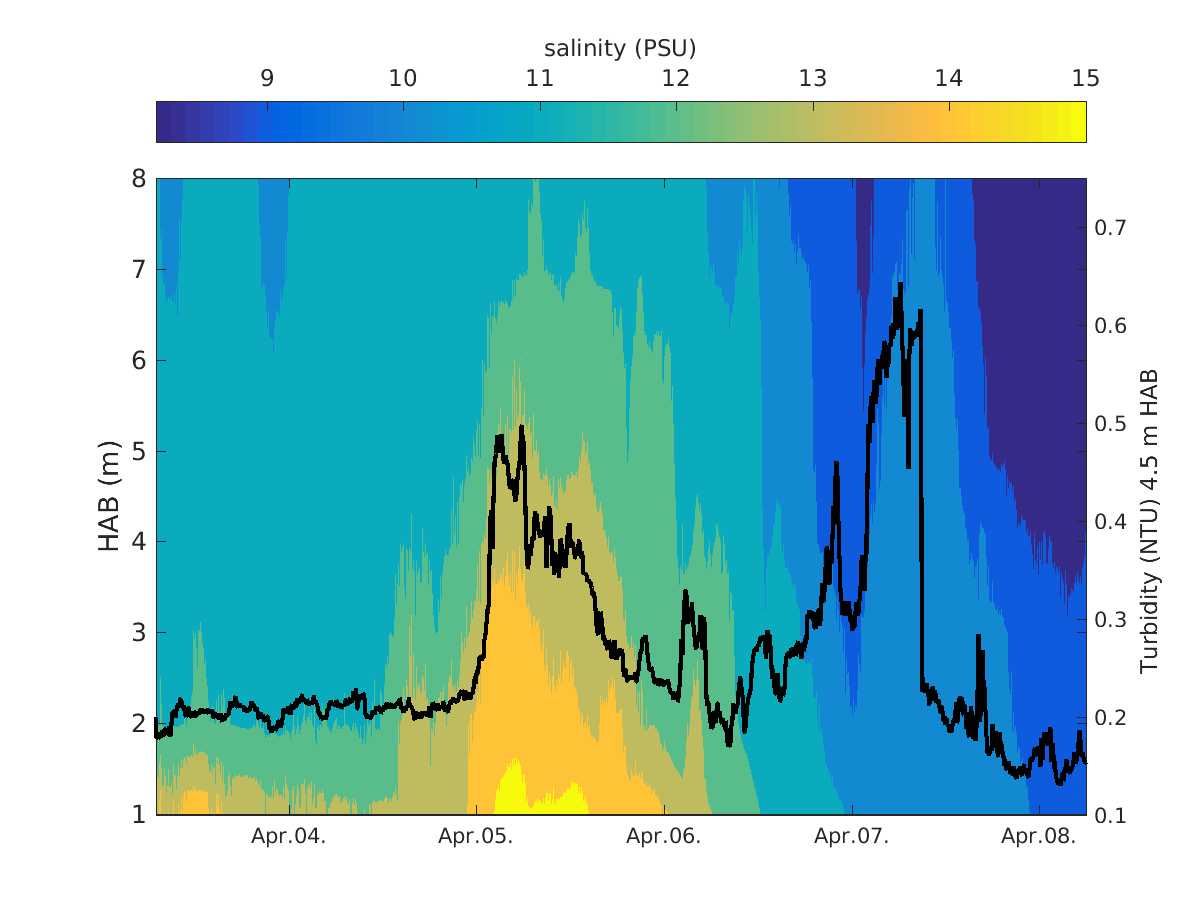
\includegraphics[width=15cm]{bilder/ctdchaintw.png}
 \caption{Salinity data obtained from the CTD Chain deployed at TW 
during cruise AL434 (see \tab{deployments}).}
 \label{ctdchain}
 \end{figure}

 
\FloatBarrier
\subsection{Basin to Coast Transect}

In \fig{transect} we see how the water body is structured along the slope from 
the coast into the basin. A sharp halocline seperates a turbulent bottom 
boundary layer (BBL) of approximately 5~m thickness from the interior. At the 
left hand side, where the slope angle steepens, the halocline is widened where 
it approaches the sea floor. 

The boundary layer is generally turbid. Turbidity is more patchy towards the 
shallow areas, but high values are confined to the bottom boundary layer, 
so no suspended matter is mixed across the halocline. This indicates that 
turbidity is caused by material originating from the sea floor and held in 
suspension by turbulent motions in the BBL.

Just like turbidity, dissipation is also enhanced in the BBL. In the area where 
the halocline encounters the sea bed on the steep slope, dissipation is 
suppressed by the high stratification. Further up the slope, right above the 
halocline, there is again an area with greatly enhanced dissipation. This 
yields that sediment could be resuspended locally when the halocline is 
advected up the slope.

Isolines of salinity (please note that salinity determines the density in this 
region) below the halocline are tilted towards the bottom, consistent with the 
observations of boundary layers over sloping topography in e.g. 
\cite{Lorkeetal2005a}. Shear induced convection and, in the presence of an 
oscillatory current, residual (upslope) sediment transport as described in 
\cite{schulzumlauf2016} is consequently within the realms of possibility here.

\begin{figure}[ht]
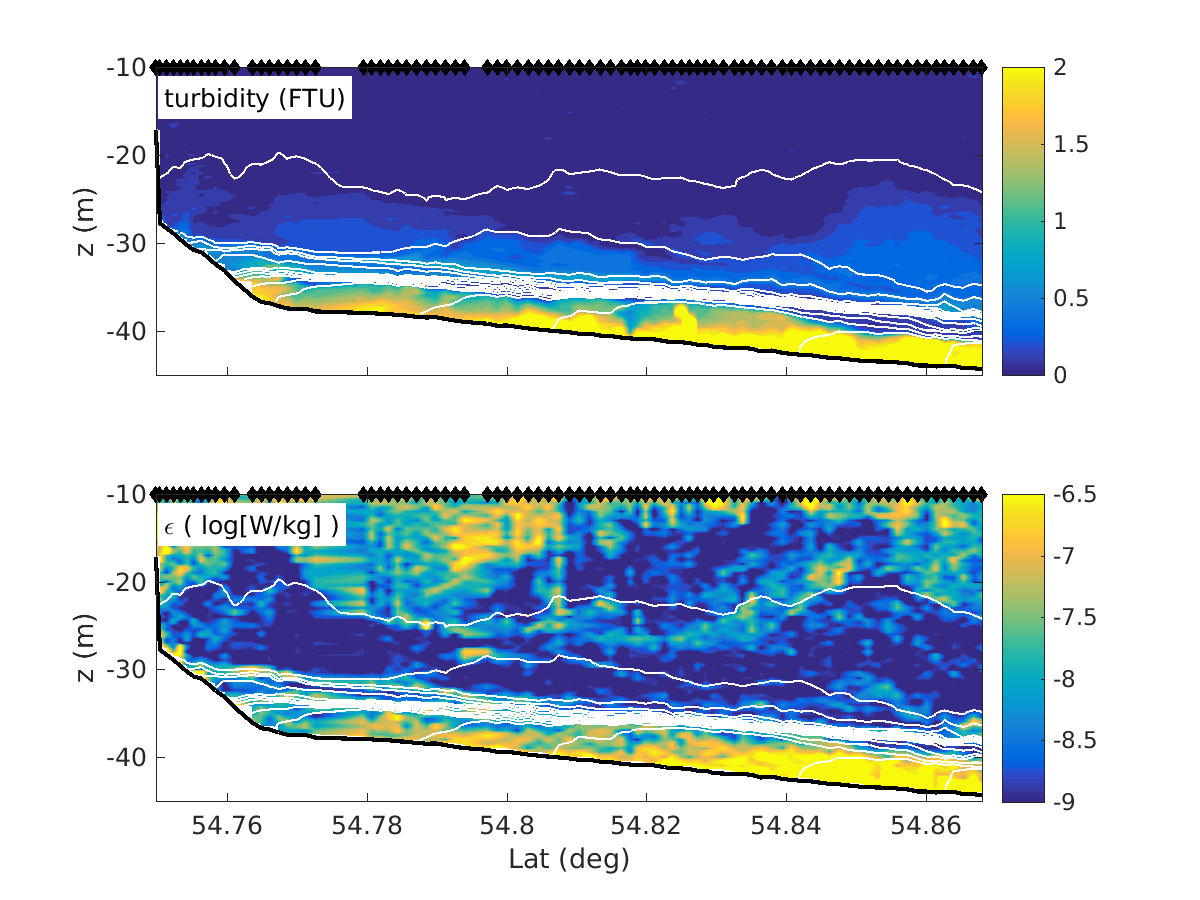
\includegraphics[width=40pc]{bilder/abtrans.png}
 \caption{Turbidity and dissipation rate from the microstructure transect T1 
in January 2016. White lines indicate levels of equal salinity.}
 \label{transect}
 \end{figure}

\FloatBarrier
\subsection{Arkona Basin}

 During each of the three cruises, we collected microstructure data in the 
Arkona Basin. \fig{abmss} shows the profiles of dissipation rate and turbidity, 
averaged over all profiles obtained in the basin for each cruise. A turbulent 
BBL is visible in all three profiles, ranging from 1 to 5 m thickness. 
Turbidity is again enhanced in the BBL, but not above, supporting the 
observation from the last section. As this data set was obtained over three 
years and in different seasons, it is most likely that this turbid, very 
sharply defined BBL is constantly present in the Arkona Basin.

   \begin{figure}[ht]
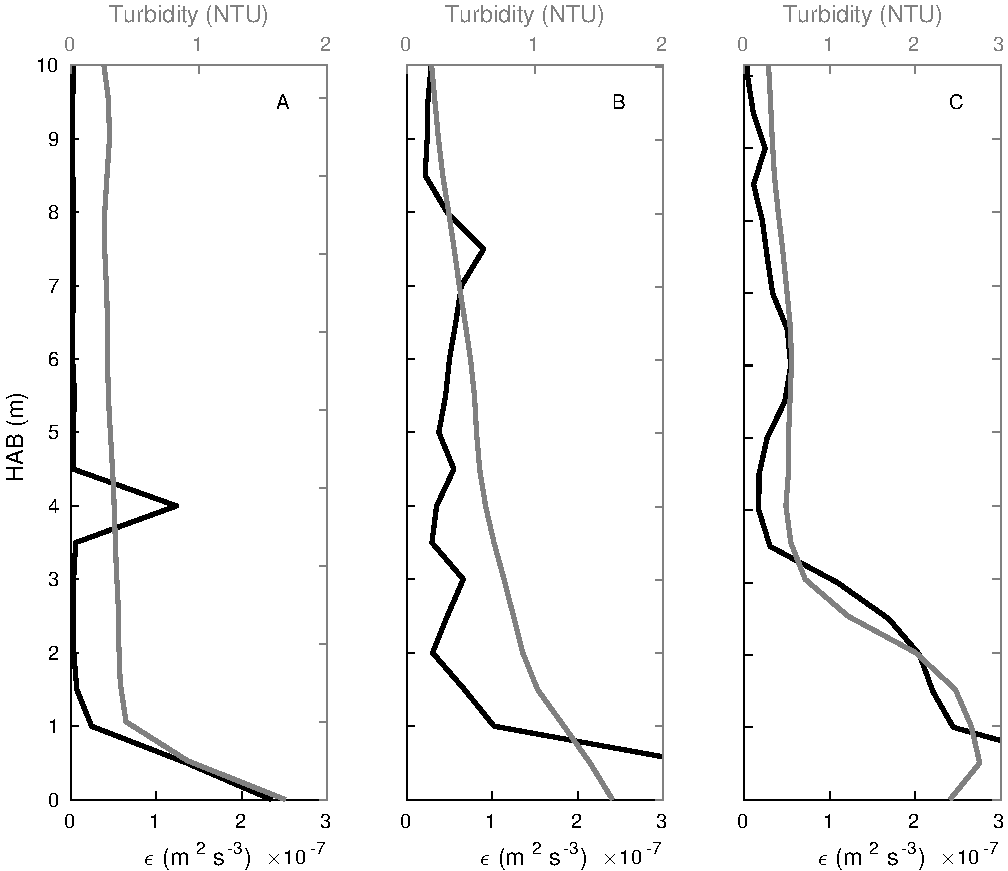
\includegraphics[width=15cm]{bilder/arkona_mss.pdf}
 \caption{Turbidity and dissipation rate from all microstructure transect in 
the Arkona Basin. Solid lines are mean values, dashed line the standard 
deviation. Only the lowermost part of the water column is displayed here.}
 \label{abmss}
 \end{figure}

The data described in the sections above yields that this reservoir of fine 
grained sediment, constantly held in suspension, can be advectively 
transported across the rim of the Arkona basin to the shallower areas well 
below 30~m. 

\section{Discussion}

This study focusses on finding processes which can transport sediment upslope 
from the deep basins back to shallower areas. We have found from the 
microstructure measurements in the Arkona basin, that in spite of the depth and 
therefore the absence of wave-induced resuspension, a layer of 
suspended fine-grained sediment is present near the bottom. This yields that 
sediment that is transported into the basin can be held in suspension there 
or can be resuspended once it is deposited there.

We furthermore found that this turbid and turbulent BBL is present everywhere 
along the slope, confined by a regional halocline. This near bottom pool of 
saline water with high concentrations of suspended matter is not in rest, but 
advected up- and down the slope by upwelling events and inertial oscillations. 
Sediment originating from the deep parts of the basin can therefore be 
transported on-shore over several kilometers. In the upwelling situation 
discussed above, the integrated near bottom velocity yielded an up slope 
transport over a distance of more than 8 kilometers in less than 24 hours. 

What can not be answered from the observations is whether suspended sediment 
that is transported up the slope settles there and a net upslope transport of 
sediment occurs. A process that induces net sediment transport across sloping 
topography is slope-induced tidal straining. The prerequisites for this 
process, namely vertical stratification, sloping topography and an oscillatory 
current, are all present in the study area. 

From the non-dimensional description of the process in \cite{schulzumlauf2016}, 
we can infer which settling velocity, and consequently which kind of sediment, 
is favored for up-slope transport. Sediment transport was found 
to be enhanced for non-dimensional settling velocities of $P= w_s \slash U = 
10^{-2}$. Here, $w_s$ is the settling velocity of suspended sediment and $U$ 
the magnitude of the oscillatory flow. Cross-slope flow velocities are in the 
order of 0.1~m~s$^{-1}$ in this region \citep[][]{lass1993}, yielding that 
sediment with a settling velocity of $w_s=10^{-3}$~m~s$^{-1}$ is favored for 
up-slope transport under the conditions investigated in this study. After 
Stokes law, this settling velocity corresponds to medium to coarse silt. As 
visible in \fig{tauberkarte}, this is exactly the sediment present in this 
area. Along the transect T1, indicated in \fig{studyarea}, sediment 
distribution ranges from fine silt in the basin to coarse silt near the shore. 
Additionally, sorting of the sediment is better near-shore than in the basin. 
Both indicates the occurrence of residual sediment transport by slope-induced 
tidal straining here.

Another indicator for sediment transport out of the basin is the distribution 
of mercury in this region. In the Arkona basin, ammunition was dumped during 
World War II. This resulted in a heavy contamination of the sediment with 
mercury. As visible in \fig{hg}, the dumping site in the eastern part of the 
Arkona Basin can be identified from mercury concentrations of over 400~$\mu$g 
kg$^{-1}$. The near bottom mean flow by saline North Sea water progressing 
through the basins is from west to east here, which explains the spreading of 
mercury to the east. The cyclonic rim current can distribute mercury 
contaminated sediment along the rim of the basin. But mercury concentrations 
are also enhanced in shallower parts of the basin, yielding that sediment is 
also transported from deeper to shallower parts, across the isobaths. One 
possible mechanism inducing this transport is slope-induced tidal straining.
   \begin{figure}[ht]
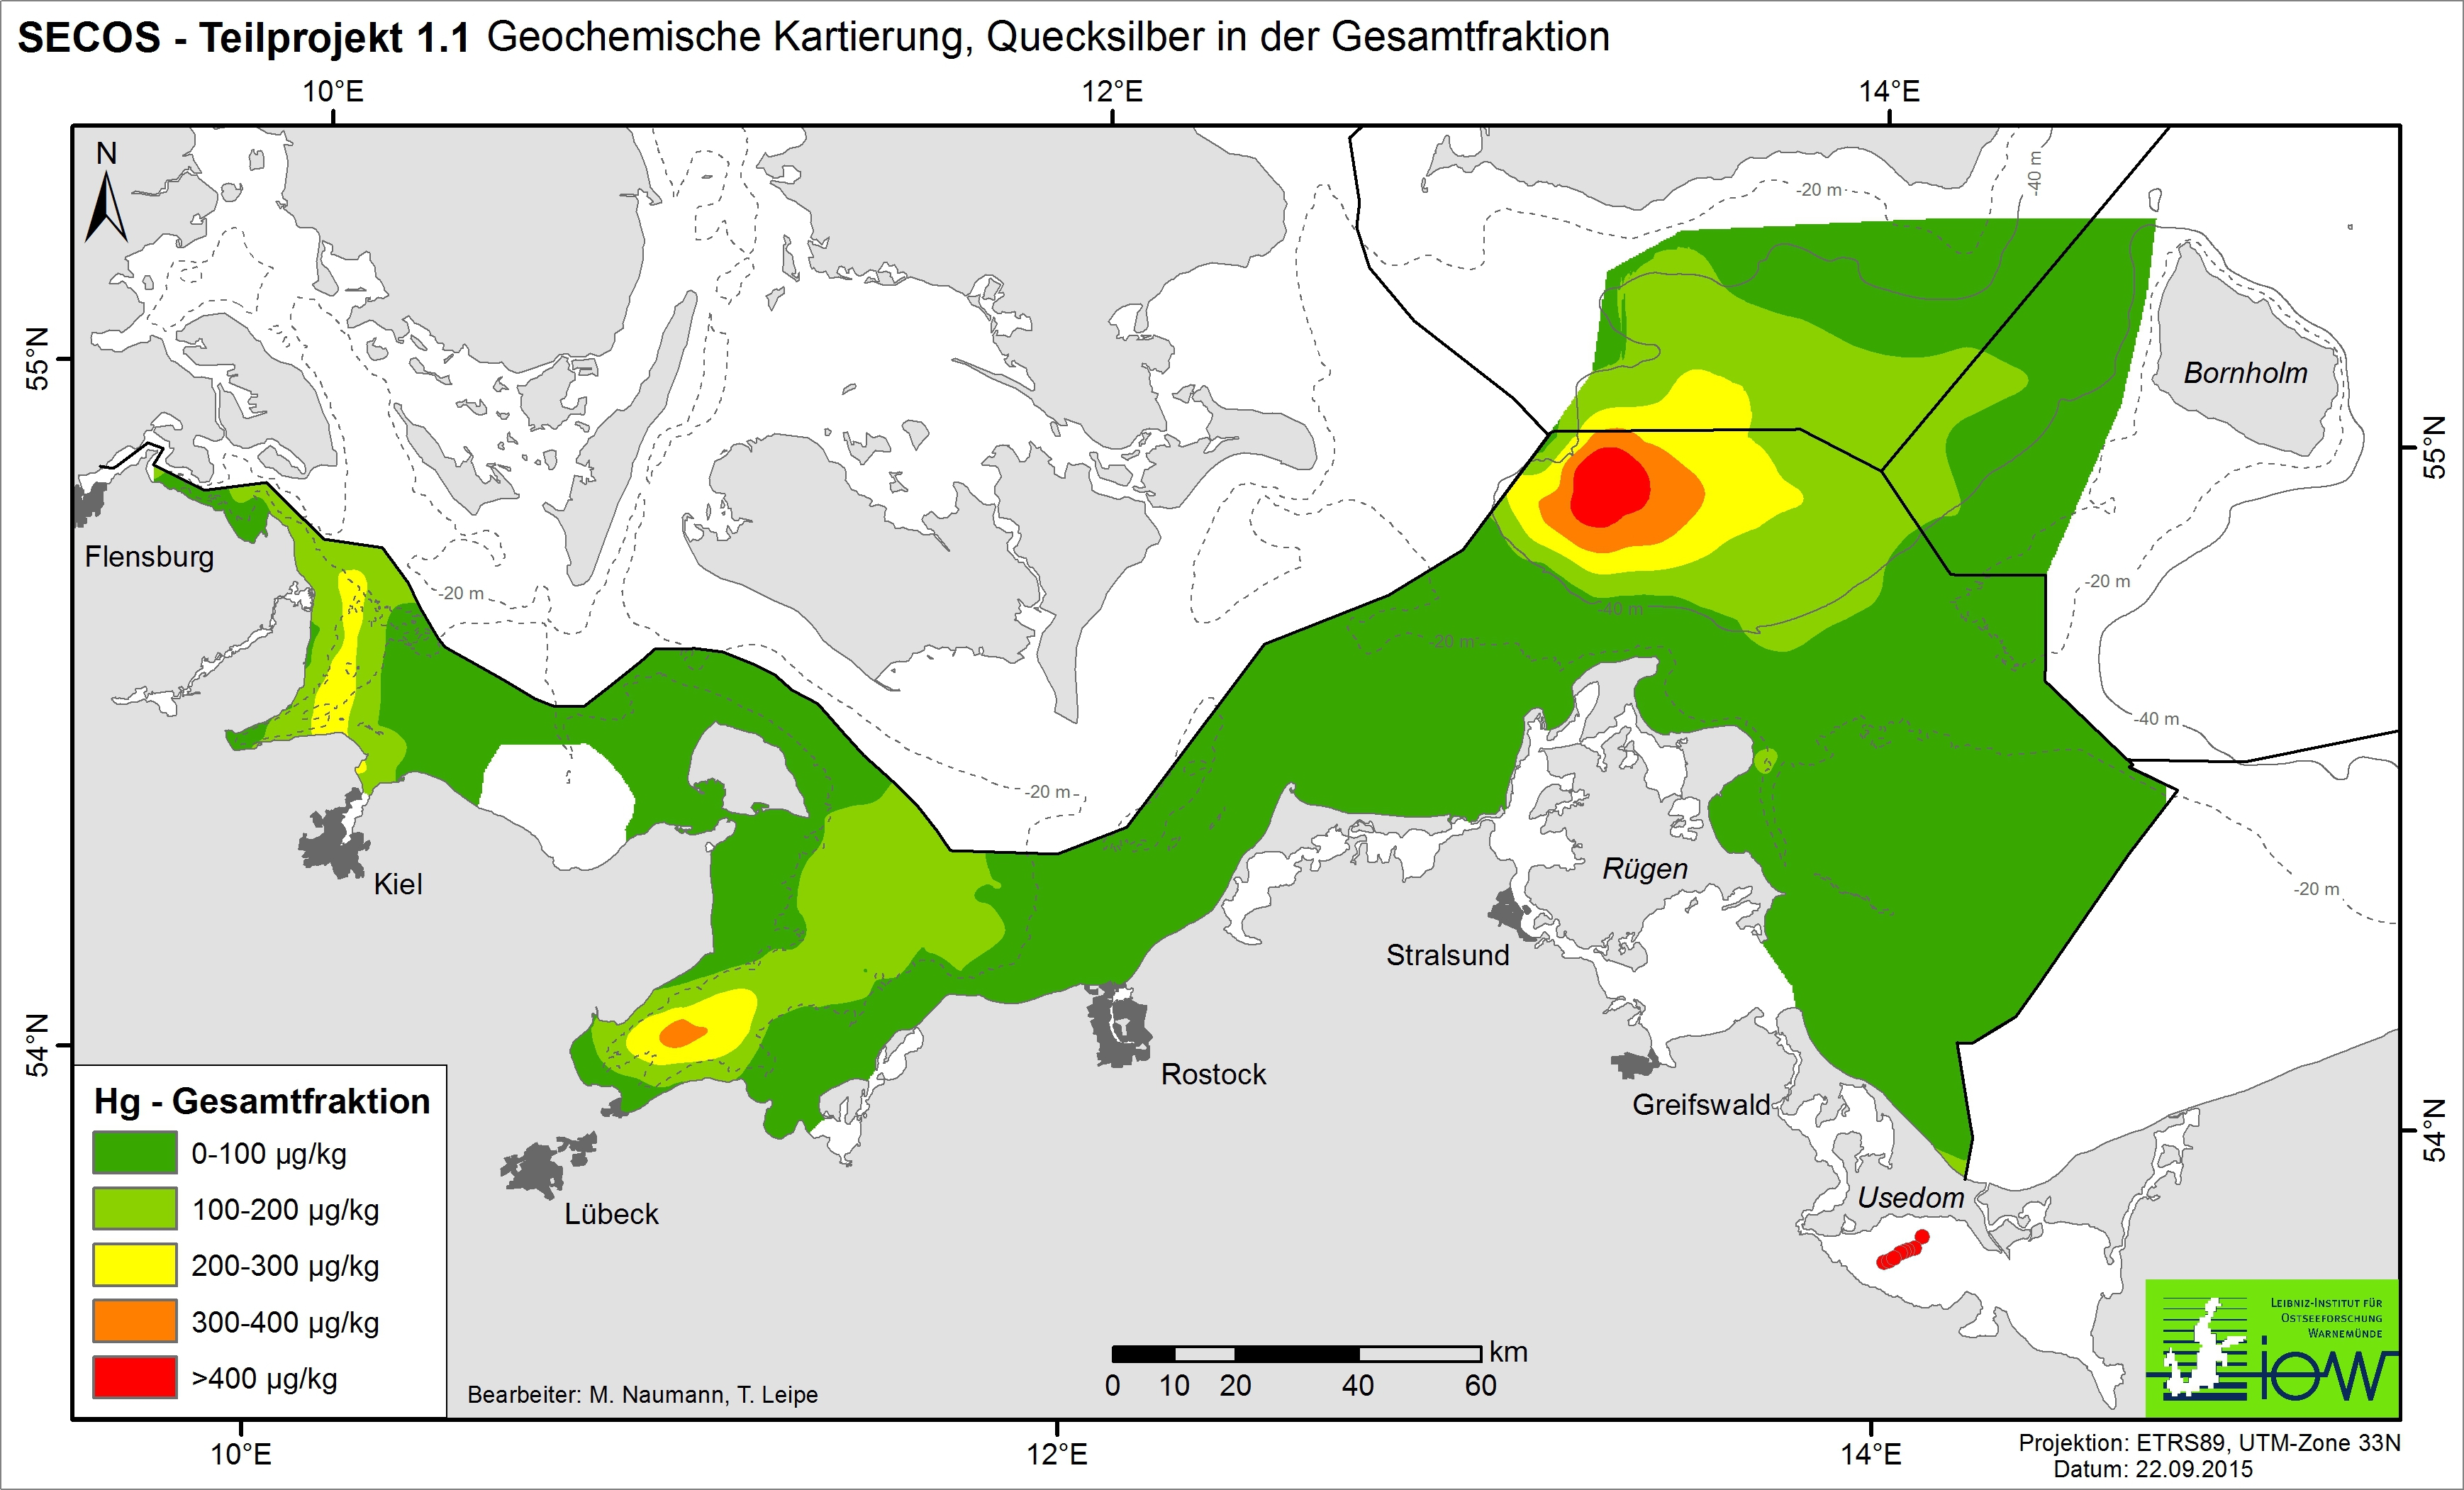
\includegraphics[width=15cm]{bilder/HG_GF.jpg}
 \caption{Mercury concentration in the sediment. Courtesy of Michael Naumann, 
reprinted with permission. [ABKLÄREN UND BESSERE KARTE?]}
 \label{hg}
 \end{figure}
 
\section{Conclusions}

One of the most important findings of this study is that sediment once 
deposited in the Arkona basin can be transported back onshore. 
This yields that fine-grained sediment from all the deep basins in the Baltic 
Sea, which are considered to be purely depositional, can be exported to 
shallower areas. This has great implications on the distribution of pollutants, 
like the mercury originating from the ammunition dumping site in the Arkona 
basin. Pollutants accumulated in the deep basins are not confined to remain 
there, but can spread towards shallower areas where they can endanger the local 
biosystem.

Several different mechanism cause sediment transport. Firstly, the mean flow of 
the dense bottom current spreads suspended sediment to the east while it 
propagates through the basin structure of the Baltic Sea. Additionally, the 
cyclonic rim current distributes sediment along the isobaths inside the basin. 
Secondly, upwelling tilts the bottom water pool towards the shore and saline 
water from the deep is advected up the basin slope, accompanied by 
suspended sediment originating from the deep parts of the basin. From the data, 
we can not determine whether this advected sediment is deposited in the 
shallower parts, or if it disappears to the deeper areas again along with the 
saline water mass. Finally, evidences are given that oscillatory currents 
in cross-slope direction, which have been identified not only in our 
observations, can cause a residual sediment transport induces by asymmetries in 
stratification and consequently vertical turbulent mixing as described in 
\cite{schulzumlauf2016}. Observed slope angle and vertical density 
stratification are well within the range which promote up-slope sediment 
transport. Sediment distribution on the transect from basin to the coast is in 
agreement with the type of sediment (characterized by sediment settling 
velocity) that would be favored for up-slope transport under the observed 
conditions. Furthermore, the results found in section \ref{kap-jgr} yield that 
a dominant along-slope velocity component, which is present here, does not 
hinder the residual up-slope sediment transport.

Even though the occurrence of residual sediment transport by slope-induced tidal 
straining can not be definitely proven from the observations, many indicators 
for this process are given. Conclusively, we can say that the transport 
mechanism described in \cite{schulzumlauf2016} is likely to take place under 
the given circumstances in the Arkona basin and can explain not only the 
spreading of mercury but also the distribution of sediment in this area.